\section{Beyond Standard Model: Leptoquarks}
\frame{\tableofcontents[currentsection]}
\begin{frame}{Beyond the Standard Modell: Leptoquarks}
    \begin{columns}
        \begin{column}{0.55\textwidth}
            \begin{itemize}
                \item Theories: supersymmetry, grand unification
                \begin{itemize}
                    \item imply: scalars with colour and different quantum numbers
                    \item [\rightarrow] Leptoquarks
                \end{itemize}
            \end{itemize}
            \begin{itemize}
                \item Leptoquarks (LQs)
                    \begin{itemize}
                        \item spin 0 or spin 1
                        \item lepton number (L) $\neq$ 0
                        \item baryon number (B) $\neq$ 0
                        \item mass $\mathcal{O}\left( TeV \right)$
                        \item Three generations of LQs:
                        \begin{itemize}
                            \item Generation X of LQs couples to Generation X of the SM
                            \item [] $X \in \{1, 2, 3 \}$
                        \end{itemize}
                        \item Coupling across generations possible
                    \end{itemize}
            \end{itemize}
        \end{column}
        \begin{column}{0.45\textwidth}
            \begin{itemize}
                \item [] Possible Leptoquarks and their quantum numbers\footnotemark
            \end{itemize}
            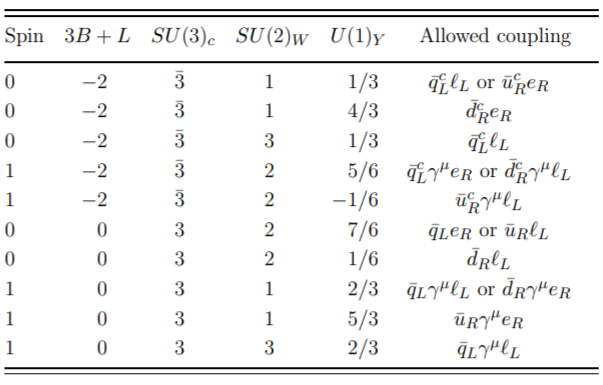
\includegraphics[scale=0.32]{content/images/LQ-Table.PNG}
        \end{column}
    \end{columns}
    \footnote[11]{Phys. Lett. B 191 (1987) 442}
\end{frame}

\begin{frame}{How LQs can contribute to $R_{K}$ and $R_{K^*}$ }
    \begin{columns}
        \begin{column}{0.6\textwidth}
            \begin{itemize}
                \item $R_{K} < 1$
                \begin{itemize}
                    \item < 2-> too many electrons
                    \item < 2-> too few muons
                    \item < 2-> combination of both?
                \end{itemize}
                \item < 3->LQs have tcouple differently to different lepton generations
            \end{itemize}
        \end{column}
        \begin{column}{0.4\textwidth}
            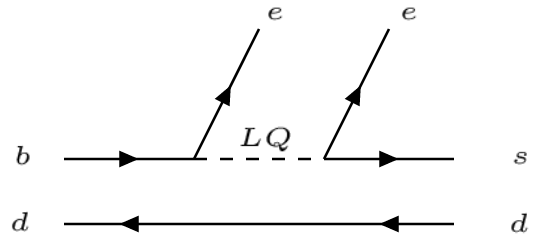
\includegraphics[width=0.7\textwidth]{content/images/LQ_ee.png}
            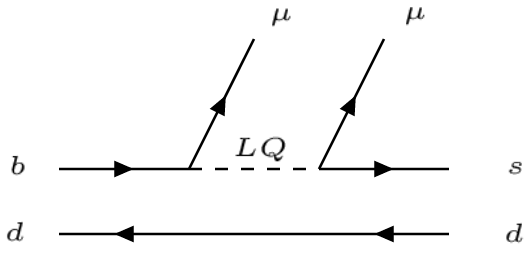
\includegraphics[width=0.7\textwidth]{content/images/LQ_mumu.png}
        \end{column}
    \end{columns}
\end{frame}
